\documentclass{beamer}
\usepackage[utf8]{inputenc}
\usepackage[T1]{fontenc}
\usepackage{graphicx}
\usepackage{color}
\usepackage{hyperref}
\usepackage[all]{xy}

\setbeamertemplate{frametitle continuation}[from second]

% \mode<presentation>
% {
%   \usetheme{Warsaw}
%   % or ...

%   \setbeamercovered{transparent}
%   % or whatever (possibly just delete it)
% }


\title{Why property-based testing matters}

\author[Pedro Vasconcelos]{Pedro Vasconcelos \\ \texttt{pbvascon@fc.up.pt}}

\institute[LIACC, DCC/FCUP]{
  DCC/FCUP \& LIACC \\
  
\includegraphics[width=0.4\textwidth]{images/fcup-identidade-logotipo-cores}
  \qquad
  \raisebox{4ex}{
\includegraphics[width=0.3\textwidth]{images/liacc-logo.png}}
}


\newcommand{\bs}{\symbol{92}}

% discard trial for counter-example
\newcommand{\counter}[1]{\textbf{#1}}
\newcommand{\noncounter}[1]{{\mathtt{#1}}}

\newcommand{\conc}{\ensuremath{\!+\!\!+}}

% If you have a file called "university-logo-filename.xxx", where xxx
% is a graphic format that can be processed by latex or pdflatex,
% resp., then you can add a logo as follows:

% \pgfdeclareimage[height=0.5cm]{university-logo}{university-logo-filename}
% \logo{\pgfuseimage{university-logo}}



% Delete this, if you do not want the table of contents to pop up atr
% the beginning of each subsection:
%\AtBeginSubsection[]
%{
%  \begin{frame}<beamer>
%    \frametitle{Overview}
%    \tableofcontents[currentsection,currentsubsection]
%  \end{frame}
%}


% If you wish to uncover everything in a step-wise fashion, uncomment
% the following command: 

%\beamerdefaultoverlayspecification{<+->}


\begin{document}

\begin{frame}
  \titlepage
\end{frame}

\begin{frame}
  \frametitle{Overview}
  
  \begin{itemize}
  \item A long-standing challenge for software engineering 
    is ensuring software correctness
  \item Formal proofs are (still) expensive and rarely used
  \item \emph{Tests} are the most commonly used
    practical technique 
  % \item \emph{Types} are another one (for another talk!)
  \item \emph{Unit tests} are the industry-standard
    for verification ``in the small''
  \end{itemize}

\end{frame}

\begin{frame}{This talk}
  
  \begin{itemize}
  \item \emph{Property-based testing}: an
    automatic testing alternative to unit tests
  \item A ``lightweight'' formal method
  \item Available for many programming languages
  \item Many successful applications in open-source and industrial
    systems
  \item But still not commonly taught and under-utilized in practice
  \item Slides and demo code: \url{https://github.com/pbv/why-pbt-matters}  \end{itemize}


  
\end{frame}

\begin{frame}[fragile]
  \frametitle{Unit tests}
\begin{itemize}
\item Code fragments for testing functions, classes, libraries, etc.
\item Express the expected outputs for specific combinations of inputs
\item Example: testing an integer square root function in Python
\begin{verbatim}
def test_isqrt():
   assert isqrt(0) == 0
   assert isqrt(2) == 1
   assert isqrt(4) == 2
   assert isqrt(5) == 2
   assert isqrt(9) == 3
\end{verbatim}
\end{itemize}


\end{frame}


\begin{frame}[fragile]
  \frametitle{Problems with unit tests}

  Cognitive bias:
  \begin{itemize}
  \item how can we include an edge case in the tests
    that we didn't consider in the code?
  \end{itemize}
  \medskip
  
  Poor scaling:
  \begin{itemize}
  \item a few unit tests per feature
  \item for $n$ features, $O(n)$ unit tests
  \item but testing \emph{interactions} between features requires $O(n^2),
    O(n^3), \ldots$ unit tests
  \end{itemize}
  \pause
  \bigskip
  

    \begin{minipage}{0.6\textwidth}
      Solution:
      \medskip
      
      \begin{quote}
        ``Don't write tests \\
        --- generate them!''
      \end{quote}
      John Hughes, co-author of the \emph{QuickCheck}
      PBT library
    \end{minipage}
    \begin{minipage}{0.3\textwidth}
      \hfill
      
\includegraphics[width=0.8\textwidth]{images/john-hughes}
    \end{minipage}
  
\end{frame}

\begin{frame}[allowframebreaks]
  \frametitle{Property-based testing}

\begin{itemize}
\item Write \emph{properties} instead of specific tests
\begin{itemize}
\item should be universal, i.e.\@ hold for all values
\item should define the expected behaviour for \emph{all} cases
\end{itemize}
\item Specify \emph{generators} for the inputs
\item The testings framework runs the property with
  a large number of inputs
  \begin{itemize}
  \item testing fails if a \alert{counter-example} is found
  \item otherwise, testing succeeds
  \end{itemize}
\end{itemize}

\framebreak

\begin{itemize}
\item QuickCheck (2000): first PBT library (for Haskell)
\item Implementations for other languages
  \begin{description}
  \item[PropEr] for Erlang
  \item[ScalaCheck] for Scala
%  \item[QuickCheck-Core] for OCaml
  \item[Hypothesis] for Python
  \item[FsCheck] for F\#
  \item[JUnit-QuickCheck] for Java
  \item[RapidCheck] for C++
  \end{description}
\end{itemize}
\bigskip

\ldots many others: \url{https://en.wikipedia.org/wiki/QuickCheck}
\end{frame}


\begin{frame}[fragile]
  \frametitle{Example property}

  What can we say about the integer square root function?
  \pause
  \medskip

  \begin{block}{Property}
    Let $n$ be an arbitrary non-negative number;
    let $r = \texttt{isqrt}(n)$; then
    \[ r\geq0 \land r^2 \leq n \land (r+1)^2>n  \]
    i.e.\@ $r$ should be \emph{largest non-negative integer} such that
  $r^2 \leq n$.
  \end{block}
  \pause
  \medskip

  In Python:
\begin{semiverbatim}
from hypothesis import given
import hypothesis.strategies as st
@given(\alert<5>{st.integers(min_value=0)})  \only<5->{\textsl{# non-negative integer}}
def test_isqrt(\alert<4>{n}):                \only<4->{\textsl{# for all n}}
    r = isqrt(n)
    assert \alert<6>{r>=0 and r**2<=n and (r+1)**2>n}   \only<6->{\textsl{# assertion}}
  \end{semiverbatim}

\end{frame}

\begin{frame}
  \frametitle{Properties in Hypothesis}

  \begin{itemize}
  \item Properties are \emph{functions}\ldots
  \item \ldots that should fail if the expected condition is not met
  \item Arguments are \emph{universally quantified}
  \item For each property:
    \begin{itemize}
  \item test with a large number of random tests (100 by default)
  \item generated using \emph{strategies}
  (defined by \texttt{@given})
    \end{itemize}
  \item Module \texttt{hypothesis.strategies} provides:
    \begin{itemize}
    \item \emph{predefined strategies} for basic types
    \item methods for \emph{modifying} and \emph{combining} strategies
    \end{itemize}
  \end{itemize}
\bigskip

  \hfill (Cue demo.)
\end{frame}



\begin{frame}
  \frametitle{Strategies}

  \begin{description}
  \item[integers()] generate integers
  \item[booleans()] generate logical values 
  \item[text()] generate Unicode strings
  \item[lists($s$)] lists of elements given by strategy $s$
    % \item[tuples($s1,s2,\ldots$)] lists of elements given by strategies $s1,s2,\ldots$
    \item[\ldots] many others
  \end{description}
  \bigskip
  
  We can also:
  \begin{itemize}
  \item modify strategies using \emph{parameters} (e.g.\@ \texttt{min\_value})
  \item modify strategies by \emph{mapping} and \emph{filtering}
  \item combine them using some \emph{combinator functions}
  % \item sample them using the \texttt{.example()} method    
  \end{itemize} 
\end{frame}


\begin{frame}
  \frametitle{Another example}

  Let's test the interaction between \emph{list reverse}
  and \emph{append}.
  
  Consider $x, y$ two arbitrary lists:

  \[  reverse(x + y) = \alt<1>{\hspace{2ex}???\hspace{18ex}}{reverse(y) + reverse(x)} \]
  \pause

  Example:
  \[\begin{array}{ll}
      reverse([1,2] + [3,4]) &= reverse([3,4]) + reverse([1,2]) \\
                             &= [4,3] + [2,1]\\
                             &= [4,3,2,1]
  \end{array}\] 
\end{frame}

\begin{frame}[fragile]
  \frametitle{Testing with lists of integers}

\begin{verbatim}
intlist = st.lists(st.integers())
@given(intlist, intlist)
def test_reverse_append(x, y):
    assert reverse(x + y) == reverse(x) + reverse(y)
\end{verbatim}
\medskip
\pause
  
\begin{semiverbatim}
$ pytest basic.py -k test_reverse_append

==================== FAILURES ==========================
\alert{______________ test_reverse_append _____________________}

x = [0], y = [1]
\end{semiverbatim}
What happened\ldots ?  
\end{frame}

\begin{frame}[fragile]
  \frametitle{Checking expectations}


\begin{itemize}
\item We've written the property incorrectly!
\begin{semiverbatim}
  assert reverse(x + y) == reverse(\alert{x}) + reverse(\alert{y})
      \textsf{instead of}
  assert reverse(x + y) == reverse(y) + reverse(x)  
\end{semiverbatim}
\item Hypothesis found a counter-example for the wrong property:
   \[ reverse([0]+[1]) \neq reverse([0]) + reverse([1]) \]
\item This is the \emph{smallest} counter-example
  that falsifies the property
\item Hypothesis \emph{always} find this counter-example
  (regardless of random generation)!
\end{itemize}
\end{frame}

\begin{frame}[fragile,allowframebreaks]
  \frametitle{Shrinking}

Assume Hypothesis randomly generates
\begin{semiverbatim}
x = [2,2]
y = [1]
\end{semiverbatim}
This is a counter-example because:
\begin{semiverbatim}
      reverse([2,2]+[1]) \ensuremath{\neq}  reverse([2,2]) + reverse([1])
\end{semiverbatim}
\medskip

Hypothesis attempts to simplify
the counter-example (``shrinking'')
before presenting:
\begin{itemize}
\item removing elements from the lists
\item recursively shrinking the elements inside the lists
\end{itemize}
This is very useful to reduce ``noise'' from the randomly generated data.
\end{frame}

\begin{frame}
\frametitle{Shrinking in action}

\[ \xymatrix@-0.5pc{
 & \counter{[2,2],[1]}\ar[dl]\ar[d] \\
 \noncounter{[],[1]} &  \counter{[2],[1]}\ar[dl]\ar[dr] \\
 \noncounter{[],[1]} & &\alert<2->{\counter{[0],[1]}}\ar[dl]\ar[d]\ar[dr]
 &  \visible<2->{\alert{\text{minimal}}} \\
&  \noncounter{[],[1]} & \noncounter{[0],[]} & \noncounter{[0],[0]}
} 
\]

\begin{itemize}
\item Shrinking ends with  \texttt{x = [0]}, \texttt{y = [1]}
  (smaller lists are no longer counter-examples)
\item For this property this is \emph{minimal} counter-example
\item In general, shrinking only finds a \emph{local minimum}
\end{itemize}
\end{frame}


\begin{frame}[allowframebreaks]
  \frametitle{Validating AI generated code}

    \begin{center}
\includegraphics[width=0.75\textwidth]{images/rle_chat.png}
  \end{center}
  
  \begin{itemize}
  \item Let us use Hypothesis to validate AI generated code
  \item Problem: write a pair of encode/decode functions
    for \alert{run-length encoding}   
  \end{itemize}

  \[ \xymatrix@-0.5pc {
      \texttt{'AABBCAAAAA'}\ar@/^/[rr]^{encode} &
      & \texttt{'A3B2C1A5'}\ar@/^/[ll]^{decode}
    }
  \]

\end{frame}

\begin{frame}[fragile]
  \frametitle{Testing ChatGPT solution}

  \begin{block}{``Roundtrip'' property}
\begin{verbatim}
@given(st.text())
def test_decode_encode_1(s):
    assert rle_decode(rle_encode(s)) == s
\end{verbatim}
    \end{block}\pause


\begin{semiverbatim}
$ pytest rle_tests.py -k test_decode_encode_1
=================== FAILURES ===========================
\alert{_____________ test_decode_encode_1 _____________________}

s = '01'
\end{semiverbatim}

The solution doesn't work for (some) strings with digits!
  
\end{frame}

\begin{frame}[fragile]
  \frametitle{Characterizing failure}

  We can check if the generated code
  works when the string contains no digits:
\begin{verbatim}
nodigits = st.characters(exclude_categories=('Nd','Nl','No'))
@given(st.text(alphabet=nodigits))
def test_decode_encode_2(s):
    assert rle_decode(rle_encode(s)) == s
\end{verbatim}

  \begin{itemize}
  \item The property now passes the default 100 tests
  \item We can now:
    \begin{itemize}
    \item try to fix the solution for digits 
    \item perform statistics on test data
    \item improve test data distribution
    \end{itemize}
  \item This greatly increases the trust in the generated code
  \end{itemize}
   
\end{frame}


\begin{frame}[fragile]
\frametitle{A larger example}
\framesubtitle{Based on production code from Ericsson}

SMS text packing:
\begin{itemize}
\item 7-bit characters;
\item transmitted using 8-bit \emph{bytes};
\item we can pack eight 7-bit caracteres into seven 8~bit bytes;
\item two functions:
\begin{verbatim}
pack(seq: bytes) -> bytes
unpack(seq: bytes) -> bytes
\end{verbatim} 
\end{itemize}

\begin{itemize}
  \item John Hughes's company (QuviQ) found a subtle bug 
    affecting strings of length multiple of 8
    ending in a \texttt{\bs NUL} character
  \item The code had already been unit tested and
    was in production
  \end{itemize}
\end{frame}

\begin{frame}[allowframebreaks]
  \frametitle{Conclusion}

\begin{itemize}
\item PBT philosophy: write \emph{properties} and \emph{generate} tests
\item Lightweight: implemented as libraries
\item Flexible: domain-specific languages (DSLs) for writing
    data generators and properties
 \item Scales to realistic software
    
\item Couples executable specifications with code
\item Useful for comunicating expectations among developers
\item Useful for finding subtle bugs in complex systems 
\end{itemize}
\end{frame}

\begin{frame}
  \frametitle{Challenges}
\begin{itemize}
\item Writting \emph{effective} properties  
  \begin{itemize}
  \item teaching developers pre- and post-conditions, invariants, etc.
  \item university CS/SE courses can play a significant rôle here
  \item helping industry adopt a higher-skill technology 
  \end{itemize}
\item PBT works best with well-structured software
\item Design systems around properties and not the other way around
\item Is validation of AI~generated code a ``killer app''
  for PBT? 
\end{itemize}
\end{frame}

\begin{frame}
  \frametitle{References}

  \begin{thebibliography}{9}
  \bibitem{quickheck} Koen Claessen and John Hughes.
    \emph{QuickCheck: A lightweight tool for random testing of Haskell
      programs}, ACM ICFP 2000
  \bibitem{hypothesis} D. R. MacIver \emph{et al}.
    \emph{Hypothesis: A new approach to property-based testing},
    The Journal of Open Source Software, 2019.
    See also \url{https://hypothesis.readthedocs.io/}
  \bibitem{telecoms} T. Arts, J. Hughes and J. Johansson
    \emph{Testing Telecoms Software with Quviq QuickCheck},
    ACM Workshop on Erlang, 2006
  \bibitem{autosar} T. Arts, J. Hughes, U. Norell and H. Svensson,
    \emph{Testing AUTOSAR software with QuickCheck}, IEEE ICSTW 2015
  \bibitem{practice} H. Goldstein, \emph{et al}. \emph{Property-Based
      Testing in Practice}, IEEE/ACM ICSE 2024
  \end{thebibliography}


\end{frame}

\begin{frame}
\begin{center}
  \Huge Extra slides
\end{center} 
\end{frame}


\begin{frame}
  \frametitle{Writing properties}

  \begin{description}
  \item[equivalence] $f(x) = f_{spec} (x)$
  e.g.\@ $f(x)$ is an optimized implementation
  and $f_{spec}(x)$ is a reference implementation.
    
  \item[idempotency] $f(f(x)) = f(x)$
  \item[roundtrip]  $g(f(x)) = x$ 
  \item[associativity] $f(x,f(y,z) = f(x,y),z)$
  \item[commutativity] $f(x,y) = f(y,x)$
  \item[right identity] $f(x,zero) = x$
  \item[left identity] $f(zero,x)= x$
  \end{description}
  \bigskip

  Hypothesis can write these kind of properties for you ---
  see \texttt{hypothesis.ghostwriter}.
  
\end{frame}

\begin{frame}[fragile]
  \frametitle{Generating data}

\begin{verbatim}
>>> integers().example()
848041

>>> lists(integers(min_value=0, max_value=100)).example()
[2, 29, 54, 66, 1, 27, 77, 81, 51, 18, 18]

>>> lists(integers().map(lambda x:x*2)).example()
[6668, -38, 1081651134, -6590]

>>> lists(integers()).map(sorted).example()
[-6913, -59, 37, 77, 90, 25088]

>>> lists(one_of(integers(), booleans())).example()
[True, True, -1318, True, True, -46, -46, True, -46]
\end{verbatim}
  
\end{frame}


\begin{frame}
  \frametitle{Stateful programs}

We can also use PBT to test programs that:
\begin{enumerate}
\item modify state;
\item read and write files;
\item use network services, databases, etc.
\end{enumerate}
\end{frame}

\begin{frame}
  \frametitle{Testing stateful programs}

\begin{itemize}
\item Generate sequences of commands
\item Specify behaviour using a functional model (state machine)
\item Compare the execution against the model
\end{itemize}

\begin{center}
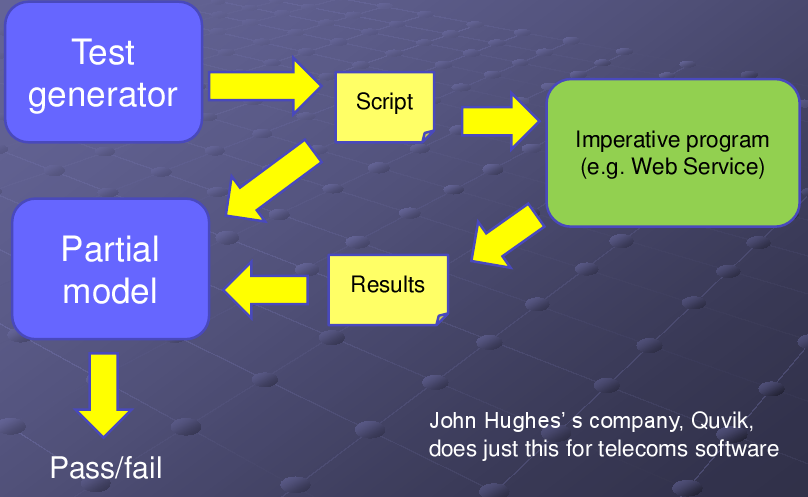
\includegraphics[width=0.75\textwidth]{images/imperative.png}
\end{center}
\end{frame}



\begin{frame}
  \frametitle{Industrial use example}

\begin{itemize}
\item Ericsson Media proxy (Java and C++)
\item Establish telephony connection throught a firewall
\item Tested with Erlang QuickCheck (Quviq.com)
\item Adding and removing participants in a call
\item Random counterexample with 160 commands
\item Shrunk automatically to 7 commands
\end{itemize}

\begin{center}
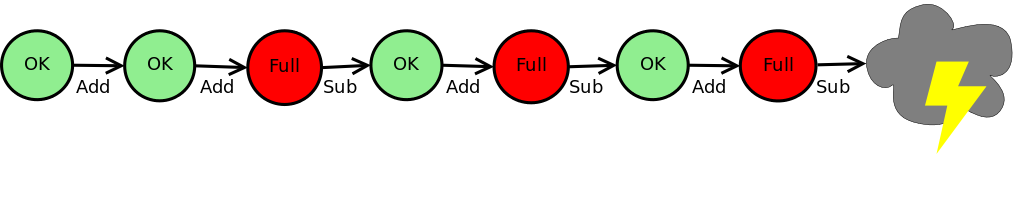
\includegraphics[width=\textwidth]{images/media1}
\end{center}
\end{frame}








\end{document}

